\section{Empirical results}
\label{sec:results}

\subsection{Basis decomposition and variance shares}
Across the $n = 1,414$ synchronized Bank Indonesia JISDOR business days from January 4, 2021 through November 12, 2026, unadjusted Indonesian rupiah prices appear systematically elevated relative to global dollar-pegged benchmarks (Table~\ref{tab:descriptive}). The BTC total basis relative to BI JISDOR ($B_t^{total}$) averages $+29.94\text{ bps}$ ($95\%$ CI $[25.73, 34.15]\text{ bps}$), with a standard deviation of $80.80\text{ bps}$, a median of $+17.09\text{ bps}$ (IQR $57.44\text{ bps}$), and $66.27\%$ positive observations. Secondary and auxiliary assets mirror this pattern: $B_t^{total}$ averages $+30.22\text{ bps}$ (SD $83.52\text{ bps}$) for ETH and $+34.96\text{ bps}$ (SD $85.76\text{ bps}$) for XRP.

\begin{table}[htbp]
\centering
\caption{Descriptive Statistics of Basis Components and Exact Variance Decomposition (bps)}
\label{tab:descriptive}
\fontsize{6.8}{8}\selectfont\setlength{\tabcolsep}{2pt}
\begingroup
\begin{tabular}{@{}>{\raggedright\arraybackslash}p{2.5cm}rrrrrrr@{}}
\toprule
Sample / Basis Series & $N$ & Mean [95\% CI] & SD & Med. & IQR & $\%>0$ & $\le$ Taker \\
\midrule
BTC Primary: B\_total & 1,414 & 29.94 [25.73, 34.15] & 80.80 & 17.09 & 57.44 & 66.3\% & 82.2\% \\
BTC Primary: B\_crypto & 1,414 & -0.83 [-2.26, 0.60] & 27.44 & -0.79 & 27.29 & 48.6\% & 97.8\% \\
BTC Primary: B\_stablecoin\_FX & 1,414 & 30.77 [26.93, 34.61] & 73.66 & 18.77 & 38.43 & 75.0\% & 88.2\% \\
BTC Primary: W\_USD\_USDT & 1,331 & -1.13 [-1.57, -0.69] & 8.17 & 0.00 & 6.60 & 48.8\% & 99.9\% \\
ETH Primary: B\_total & 1,414 & 30.22 [25.87, 34.57] & 83.52 & 16.85 & 55.55 & 67.2\% & 82.7\% \\
ETH Primary: B\_crypto & 1,414 & -0.55 [-2.02, 0.92] & 28.16 & -1.26 & 27.26 & 47.2\% & 98.0\% \\
ETH Primary: B\_stablecoin\_FX & 1,414 & 30.77 [26.93, 34.61] & 73.66 & 18.77 & 38.43 & 75.0\% & 88.2\% \\
ETH Primary: W\_USD\_USDT & 1,331 & -1.13 [-1.57, -0.69] & 8.17 & 0.00 & 6.60 & 48.8\% & 99.9\% \\
XRP Primary: B\_total & 1,414 & 34.96 [30.49, 39.43] & 85.76 & 21.22 & 56.65 & 70.6\% & 81.5\% \\
XRP Primary: B\_crypto & 1,414 & 4.19 [2.34, 6.05] & 35.60 & 2.78 & 27.72 & 55.9\% & 97.0\% \\
XRP Primary: B\_stablecoin\_FX & 1,414 & 30.77 [26.93, 34.61] & 73.66 & 18.77 & 38.43 & 75.0\% & 88.2\% \\
XRP Primary: W\_USD\_USDT & 1,331 & -1.13 [-1.57, -0.69] & 8.17 & 0.00 & 6.60 & 48.8\% & 99.9\% \\
BTC All Calendar Days: B\_total & 2,136 & 33.11 [29.52, 36.69] & 84.62 & 20.83 & 62.25 & 67.2\% & 76.1\% \\
BTC Weekends Only: B\_total & 608 & 34.47 [27.61, 41.33] & 86.25 & 26.35 & 71.29 & 67.3\% & 69.2\% \\
BTC Weekends Only: B\_crypto & 608 & -1.70 [-3.92, 0.51] & 27.84 & -0.50 & 25.03 & 49.2\% & 98.4\% \\
\bottomrule
\end{tabular}\endgroup
\begin{minipage}{\textwidth}\footnotesize\vspace{3pt}
\emph{Exact Variance Identity (BTC, $n=1,414$):} $\mathrm{Var}(B^{total}) = 6529.03$ = $\mathrm{Var}(B^{crypto})\ (752.98,\ 11.53\%)$ + $\mathrm{Var}(B^{stable\text{-}FX})\ (5425.67,\ 83.10\%)$ + $2\mathrm{Cov}\,(350.38,\ 5.37\%)$. \emph{Dynamic Fee Band Containment (BTC $B^{crypto}$):} 64.57\% inside Route A maker band; 98.44\% inside Route A taker band; 98.94\% inside Route B taker band.
\end{minipage}
\end{table}


Separating currency conversion via local \texttt{USDT/IDR} accounts for the bulk of that premium. Once expressed in \texttt{USDT} using Indodax's synchronized \texttt{USDT/IDR} book, mean BTC pure-crypto basis ($B_t^{crypto}$) falls to $-0.83\text{ bps}$ ($95\%$ CI $[-2.26, +0.60]\text{ bps}$, SD $27.44\text{ bps}$, median $-0.79\text{ bps}$), which is statistically indistinguishable from zero at the $5\%$ level. ETH behaves identically ($B_t^{crypto}$ mean $-0.55\text{ bps}$, $95\%$ CI $[-2.02, +0.92]\text{ bps}$), while XRP shows a modest positive mean of $+4.19\text{ bps}$ (SD $35.60\text{ bps}$) alongside thinner domestic ask-to-bid symmetry ($17.31\text{ bps}$ snapshot round-trip spread at $\$1\text{k}$ on November 13, 2026). By contrast, the common domestic stablecoin--FX leg $B_t^{stablecoin\text{-}FX} = 10^4(\ln U_t^{IDR/USDT} - \ln S_t^{IDR/USD})$ averages $+30.77\text{ bps}$ ($95\%$ CI $[26.93, 34.61]\text{ bps}$, SD $73.66\text{ bps}$) and is positive on $75.04\%$ of business days. Over the $n = 1,331$ overlapping days after Coinbase \texttt{USDT-USD} launched on May 4, 2021, the external stablecoin peg wedge $W_t^{USD/USDT}$ averages $-1.13\text{ bps}$ (SD $8.17\text{ bps}$, median $0.00\text{ bps}$). Offshore USD-to-USDT drift therefore plays a secondary role except during transient stress events such as the $-171.46\text{ bps}$ low around March 2023.

\begin{figure}[htbp]
  \centering
  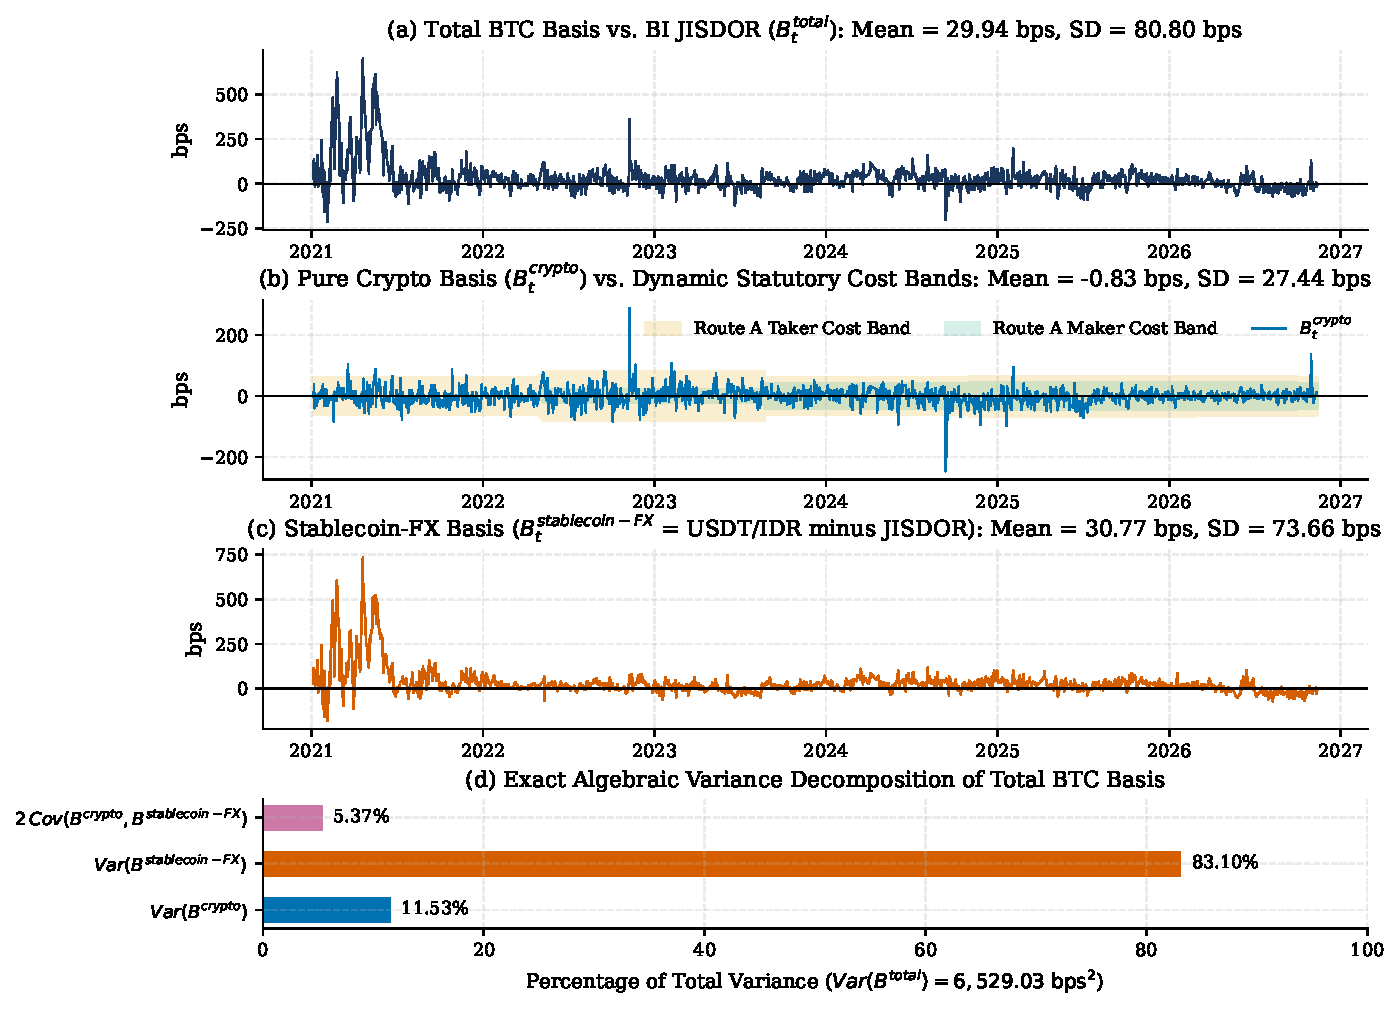
\includegraphics[width=\textwidth]{fig3_basis_decomposition.pdf}
  \caption{Two-leg basis decomposition for BTC from January 2021 through November 2026 ($n=1,414$ JISDOR business days), displaying $B_t^{total}$, $B_t^{crypto}$ inside dynamic domestic Route A taker cost bands, and the domestic stablecoin--FX basis $B_t^{stablecoin\text{-}FX}$.}
  \label{fig:decomp}
\end{figure}

The variance identity in Equation~\eqref{eq:vardecomp} shows which leg carries the movement in the total basis. For BTC, total basis variance $\mathrm{Var}(B_t^{total}) = 6,529.03\text{ bps}^2$ splits into $83.10\%$ for $\mathrm{Var}(B_t^{stablecoin\text{-}FX}) = 5,425.67\text{ bps}^2$, $11.53\%$ for $\mathrm{Var}(B_t^{crypto}) = 752.98\text{ bps}^2$, and $5.37\%$ for twice their covariance ($2\mathrm{Cov} = 350.38\text{ bps}^2$, contemporaneous correlation $0.0867$; identity discrepancy $9.1\times 10^{-13}\text{ bps}^2$). ETH and XRP show similar shares: $77.78\%$ versus $11.37\%$ for ETH ($10.85\%$ covariance), and $73.77\%$ versus $17.23\%$ for XRP ($9.00\%$ covariance). Figure~\ref{fig:decomp} plots the BTC basis series against time-varying domestic taker bands, and Figure~\ref{fig:dist} compares empirical distributions across all three cryptocurrencies. Evaluated date-by-date against regime-specific statutory taxes, CFX fees, and platform commissions (Section~\ref{sec:institutional}), $98.44\%$ of business-day BTC $B_t^{crypto}$ observations sit inside the dynamic two-leg domestic Route A taker band ($64.57\%$ inside the tighter maker band), and $98.94\%$ sit inside the cross-exchange Route B three-leg taker band. Against the fixed sample-average Route A taker threshold ($66.45\text{ bps}$, reported in the final column of Table~\ref{tab:descriptive}), containment is $97.81\%$. Across extreme interpretations of the partially verified May 2022--October 2024 Indodax fee transition ($61.0\text{ bps}$ versus $81.0\text{ bps}$ taker throughout), dynamic Route A containment stays within $[97.52\%, 98.51\%]$. Because $B_t^{crypto}$ has a standard deviation of $27.44\text{ bps}$, this high containment rate follows mechanically from its narrow dispersion relative to the $60.0$--$81.0\text{ bps}$ taker band and does not by itself prove the absence of exploitable intraday arbitrage.

\begin{figure}[htbp]
  \centering
  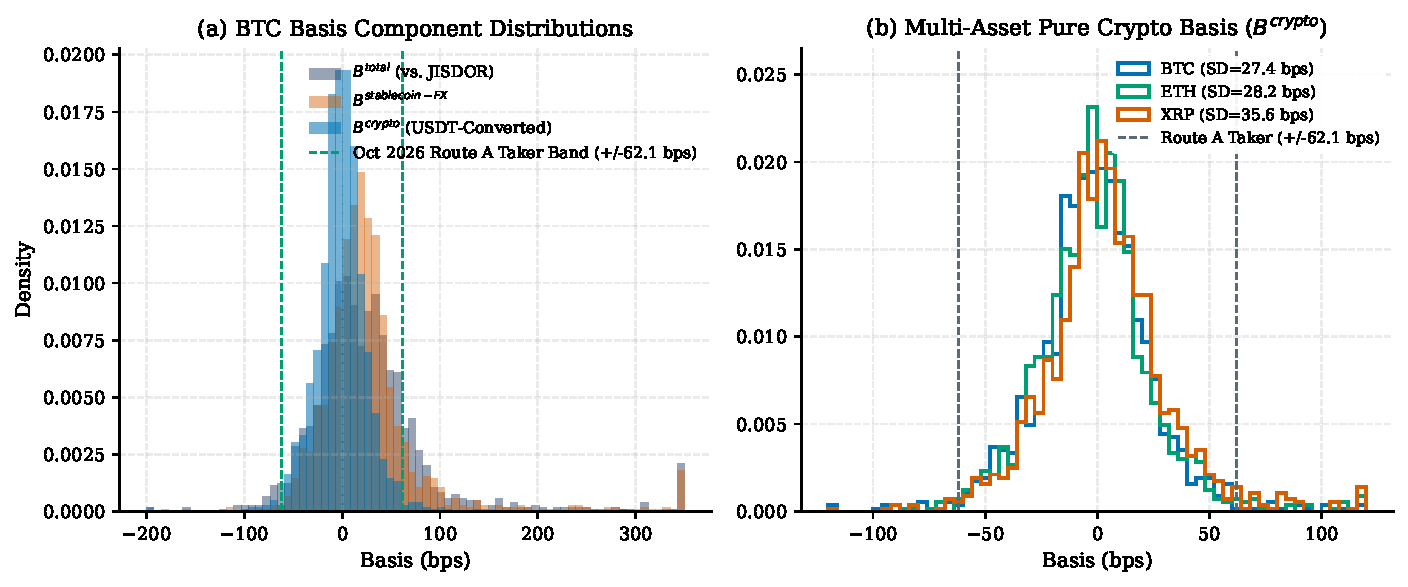
\includegraphics[width=\textwidth]{fig4_basis_distributions.pdf}
  \caption{Empirical basis distributions ($B_t^{total}$, $B_t^{crypto}$, $B_t^{stablecoin\text{-}FX}$) and multi-asset pure crypto basis ($B_t^{crypto}$) across BTC, ETH, and XRP. Extreme observations are winsorized at $[-180, 320]\text{ bps}$ in Panel~(a) and $[-120, 120]\text{ bps}$ in Panel~(b) for display.}
  \label{fig:dist}
\end{figure}

\subsection{Unit-root properties and cointegration rank}
Table~\ref{tab:unit_roots} reports ADF, Phillips--Perron, KPSS, and Zivot--Andrews single-break tests across all price levels, first differences, and basis series. Every log asset price ($\ln P_{t}^{IDR}$, $\ln P_{t}^{USDT}$) and FX benchmark ($\ln U_t^{IDR/USDT}$, $\ln S_t^{IDR/USD}$) fails to reject a unit root under ADF and PP ($p \ge 0.626$ with constant; Zivot--Andrews statistics $-3.13$ to $-3.78$ versus the $-4.80$ critical value) while rejecting KPSS stationarity ($p = 0.01$), consistent with $I(1)$ log levels and $I(0)$ first differences ($p < 0.0001$). For basis spreads, $B_t^{crypto}$ rejects a unit root ($ADF = -10.62$, $p < 0.0001$ for BTC; $-10.59$ for ETH; $-9.58$ for XRP) and fails to reject KPSS constant-mean stationarity for BTC ($\eta_\mu = 0.380$, $p = 0.086$) and ETH ($\eta_\mu = 0.383$, $p = 0.085$). By contrast, $B_t^{total}$ and $B_t^{stablecoin\text{-}FX}$ reject unit roots under ADF and PP ($p < 0.0001$) yet reject KPSS constant-mean stationarity ($\eta_\mu = 1.27$--$1.58$, $p = 0.01$). That divergence indicates level shifts in onshore stablecoin premia over 2021--2026 rather than a random walk.

\begin{table}[htbp]
\centering
\caption{Unit-root and stationarity tests (2021--2026 synchronized business-day panel)}
\label{tab:unit_roots}
\fontsize{6.6}{7.8}\selectfont\setlength{\tabcolsep}{2pt}
\begingroup
\begin{tabular}{@{}>{\raggedright\arraybackslash}p{3.4cm}rrrrrr@{}}
\toprule
Series & $N$ & ADF (Const.) & $p$-val & PP ($Z_t$) & KPSS ($\eta_\mu$) & Zivot--Andrews \\
\midrule
BTC ln P\_IDR & 1,414 & -1.072 & 0.7262 & -1.185 & 3.483 & -3.123 \\
BTC d(ln P\_IDR) & 1,413 & -15.251 & $<$0.0001 & -36.442 & 0.107 & -15.510 \\
BTC ln P\_USDT & 1,414 & -1.237 & 0.6574 & -1.317 & 3.059 & -3.163 \\
BTC d(ln P\_USDT) & 1,413 & -37.176 & $<$0.0001 & -37.226 & 0.104 & -37.349 \\
Indodax ln U\_IDR (USDT/IDR) & 1,414 & -0.356 & 0.9171 & -0.622 & 4.998 & -3.680 \\
Indodax d(ln U\_IDR) & 1,413 & -12.156 & $<$0.0001 & -39.452 & 0.050 & -13.893 \\
BI JISDOR ln S\_FX & 1,414 & -0.268 & 0.9300 & -0.385 & 5.044 & -3.782 \\
BI JISDOR d(ln S\_FX) & 1,413 & -13.093 & $<$0.0001 & -34.045 & 0.060 & -13.226 \\
BTC B\_total (bps) & 1,414 & -5.348 & $<$0.0001 & -16.339 & 1.316 & -7.319 \\
BTC B\_crypto (bps) & 1,414 & -10.280 & $<$0.0001 & -31.971 & 0.383 & -11.028 \\
BTC B\_stablecoin\_FX (bps) & 1,414 & -4.878 & $<$0.0001 & -12.102 & 1.271 & -7.402 \\
ETH B\_total (bps) & 1,414 & -5.290 & $<$0.0001 & -16.947 & 1.295 & -7.389 \\
ETH B\_crypto (bps) & 1,414 & -10.718 & $<$0.0001 & -31.316 & 0.418 & -11.273 \\
XRP B\_total (bps) & 1,414 & -6.186 & $<$0.0001 & -19.444 & 1.648 & -7.527 \\
XRP B\_crypto (bps) & 1,414 & -32.630 & $<$0.0001 & -34.761 & 2.465 & -33.617 \\
\bottomrule
\end{tabular}\endgroup
\begin{minipage}{\textwidth}\footnotesize\vspace{3pt}
\emph{Notes:} 5\% critical values: ADF constant $-2.864$, KPSS constant $0.463$ ($H_0$: stationarity), Zivot--Andrews single-break $-4.80$. All log price levels and FX series are $I(1)$; first differences and all basis spreads reject a unit root at $p < 0.0001$.
\end{minipage}
\end{table}


Table~\ref{tab:cointegration} demonstrates how omitting FX conversion reverses cointegration conclusions. Pairing Indodax \texttt{BTC/IDR} with unconverted Binance \texttt{BTC/USDT} fails every test for long-run equilibrium: Engle--Granger yields $t = -1.10$ ($p = 0.881$), Fixed-$(1,-1)$ ADF yields $-0.40$ ($p = 0.909$), Reinsel--Ahn Johansen trace is $6.33$ (far below both the $15.49$ asymptotic and $15.54$ Cheung--Lai $5\%$ critical values), and the $B = 9,999$ null-imposed restricted-VECM block-wild bootstrap ($b = 6$) returns $p_{boot} = 0.8584$. Unadjusted ETH ($\text{Trace}_{RA} = 11.20$, $p_{boot} = 0.4774$) and XRP ($\text{Trace}_{RA} = 8.38$, $p_{boot} = 0.7734$) fail identically.

\begin{table}[htbp]
\centering
\caption{Engle--Granger, Fixed-$(1,-1)$, Johansen (Reinsel--Ahn), and Bootstrap Cointegration Tests ($B=9,999$)}
\label{tab:cointegration}
\fontsize{6.3}{7.5}\selectfont\setlength{\tabcolsep}{2pt}
\begingroup
\begin{tabular}{@{}>{\raggedright\arraybackslash}p{2.5cm}rrrrrrr@{}}
\toprule
Specification & $T_{eff}$ & EG $\hat{\beta}$ & EG $t$ & Fixed ADF & Trace (RA) & MaxEig (RA) & Boot $p$ \\
\midrule
BTC Unadjusted & 1,412 & 1.0702 & -1.10 & -0.40 & 6.33 & 5.75 & 0.7314 \\
BTC JISDOR & 1,412 & 0.9993 & -4.42 & -5.37 & 151.72 & 150.32 & $\le$0.0001 \\
BTC USDT & 1,412 & 0.9994 & -10.97 & -10.62 & 513.96 & 512.73 & $\le$0.0001 \\
BTC SpotFX & 1,249 & 1.0003 & -4.81 & -6.73 & 151.09 & 149.66 & $\le$0.0001 \\
USDT IDR vs JISDOR & 1,412 & 0.9673 & -4.65 & -4.89 & 102.68 & 102.55 & $\le$0.0001 \\
ETH Unadjusted & 1,412 & 1.0161 & -0.60 & -0.44 & 11.20 & 9.11 & 0.2821 \\
ETH JISDOR & 1,412 & 0.9998 & -4.28 & -5.27 & 141.46 & 132.40 & $\le$0.0001 \\
ETH USDT & 1,412 & 0.9996 & -10.53 & -10.59 & 511.04 & 502.18 & $\le$0.0001 \\
XRP Unadjusted & 1,412 & 1.0523 & -0.86 & -0.40 & 8.38 & 6.09 & 0.5280 \\
XRP JISDOR & 1,412 & 0.9994 & -4.14 & -5.16 & 131.12 & 126.46 & $\le$0.0001 \\
XRP USDT & 1,412 & 0.9993 & -9.94 & -9.58 & 492.91 & 488.34 & $\le$0.0001 \\
\midrule
\multicolumn{8}{@{}l}{\textbf{Monte Carlo Validation of Null-Imposed VECM Bootstrap Size \& Power ($n_{MC}=150$, $B=299$):}} \\
DGP $T=25$, $r=0$ (Size) & \multicolumn{2}{r}{Asymp: 16.7\%} & \multicolumn{2}{r}{RA: 6.7\%} & \multicolumn{3}{r}{Bootstrap: 3.3\%} \\
DGP $T=25$, $r=1$ (Power) & \multicolumn{2}{r}{Asymp: 37.3\%} & \multicolumn{2}{r}{RA: 14.0\%} & \multicolumn{3}{r}{Bootstrap: 10.0\%} \\
DGP $T=100$, $r=0$ (Size) & \multicolumn{2}{r}{Asymp: 11.3\%} & \multicolumn{2}{r}{RA: 8.7\%} & \multicolumn{3}{r}{Bootstrap: 4.0\%} \\
DGP $T=100$, $r=1$ (Power) & \multicolumn{2}{r}{Asymp: 90.7\%} & \multicolumn{2}{r}{RA: 86.7\%} & \multicolumn{3}{r}{Bootstrap: 76.0\%} \\
DGP $T=500$, $r=0$ (Size) & \multicolumn{2}{r}{Asymp: 12.0\%} & \multicolumn{2}{r}{RA: 11.3\%} & \multicolumn{3}{r}{Bootstrap: 6.0\%} \\
DGP $T=500$, $r=1$ (Power) & \multicolumn{2}{r}{Asymp: 100.0\%} & \multicolumn{2}{r}{RA: 100.0\%} & \multicolumn{3}{r}{Bootstrap: 100.0\%} \\
\bottomrule
\end{tabular}\endgroup
\begin{minipage}{\textwidth}\footnotesize\vspace{3pt}
\emph{Notes:} 5\% critical values: Engle--Granger $-3.340$; Fixed-$(1,-1)$ ADF $-2.864$; Johansen asymptotic Trace $15.49$, MaxEig $14.26$ (Cheung--Lai 5\% CV at $T_{eff}=1,412$: Trace $15.54$, MaxEig $14.30$). Null-imposed restricted-VECM i.i.d. residual bootstrap uses $B=9,999$ replications.
\end{minipage}
\end{table}


Introducing synchronized currency conversion overturns those null results cleanly. Converting global \texttt{BTC/USDT} at BI JISDOR raises the Reinsel--Ahn trace statistic from $6.33$ to $151.72$ ($p_{boot} = 0.0001$, Engle--Granger $\hat{\beta} = 0.9993$, $t = -4.42$, $p = 0.0016$, Fixed-$(1,-1)$ ADF $-5.37$, $p < 0.0001$). Converting instead via domestic \texttt{USDT/IDR} raises the trace statistic further to $513.96$ ($p_{boot} = 0.0001$, Fixed ADF $-10.62$) because local crypto pairs and the domestic stablecoin leg move tightly together. Both ETH ($\text{Trace}_{RA} = 141.46$ JISDOR, $511.04$ USDT, $p_{boot} = 0.0001$) and XRP ($\text{Trace}_{RA} = 131.12$ JISDOR, $492.91$ USDT, $p_{boot} = 0.0001$) yield identical rank $r=1$ findings, and domestic \texttt{USDT/IDR} itself is cointegrated with BI JISDOR ($\text{Trace}_{RA} = 102.68$, block-wild $p_{boot} = 0.0005$ against a $5\%$ bootstrap critical value of $46.65$, $\hat{\beta}_{EG} = 0.9673$). No rank-$2$ trace test exceeds its $5\%$ critical value for BTC ($1.41$ and $1.24$ versus $3.84$), which is consistent with a single common stochastic trend. Appendix Table~\ref{tab:boot_mc} validates the block-wild bootstrap across $n_{MC} = 1,000$ replications under GARCH(1,1) and AR(1) innovations. Figure~\ref{fig:rolling} illustrates 60-business-day rolling basis averages, rolling volatility (standard deviation), and rolling cross-leg correlations through 2021--2026.

\begin{figure}[htbp]
  \centering
  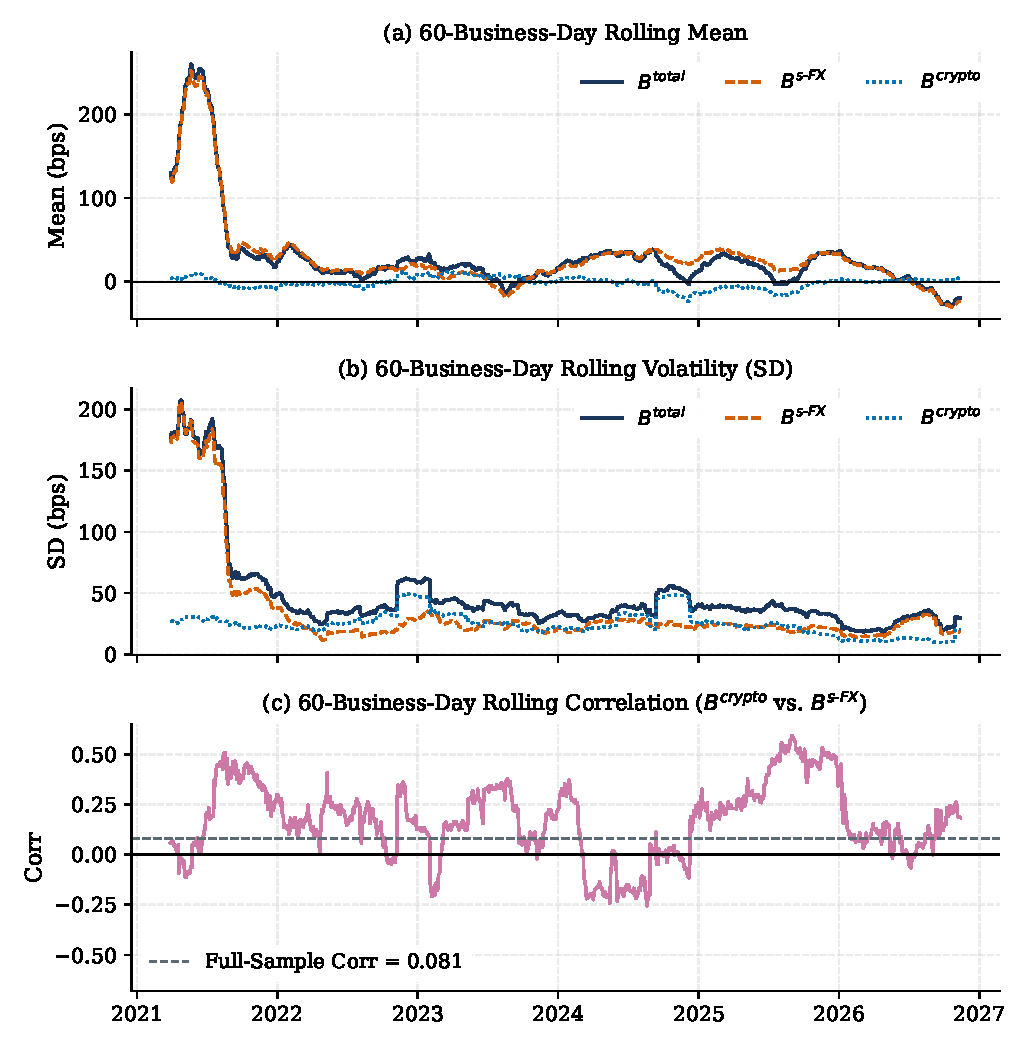
\includegraphics[width=\textwidth]{fig5_rolling_dynamics_and_corr.pdf}
  \caption{Rolling 60-business-day BTC basis means, volatility (SD), and cross-leg correlation between $B_t^{crypto}$ and $B_t^{stablecoin\text{-}FX}$ (2021--2026).}
  \label{fig:rolling}
\end{figure}

\subsection{Error-correction speeds, three-variable intraday price discovery, and threshold dynamics}
Table~\ref{tab:vecm_ecm} reports VECM estimates (Panel A daily business-day bivariate systems; Panel B five-minute 24/7 three-variable BTC systems), and Figure~\ref{fig:ec} contrasts Johansen trace statistics and daily adjustment speeds. On the synchronized daily panel ($T_{eff} = 1,412$, one lagged difference, HAC $L = 5$), Indodax BTC absorbs the error-correction burden against JISDOR-converted global BTC ($\hat{\alpha}_{local} = -0.398$, HAC SE $0.165$, $p = 0.0158$), while we fail to reject weak exogeneity for global BTC ($\hat{\alpha}_{global} = -0.213$, HAC SE $0.195$, $p = 0.2728$; LR weak-exogeneity $p = 0.092$). Accounting for full-VECM companion dynamics rather than $\alpha_{local}$ alone yields a native companion-root half-life of $3.66$ business days ($|\lambda_{\max}| = 0.8275$). Converting global BTC at domestic \texttt{USDT/IDR} increases the local adjustment speed ($\hat{\alpha}_{local} = -0.884$, HAC $p = 0.0231$, full-system half-life $0.56$ business days). For ETH and XRP, daily $\hat{\alpha}_{local}$ estimates carry the expected negative sign ($-0.193$ to $-0.775$) but are statistically insignificant under HAC standard errors ($p = 0.148$ to $0.402$) due to noisy daily aggregation. In both daily BTC systems, cross-market innovations are nearly collinear ($\rho_u = 0.991$ and $0.997$), so daily Cholesky Hasbrouck bounds span nearly $[0, 1]$ and are uninformative. In the Indodax \texttt{USDT/IDR}--JISDOR currency system ($\rho_u = 0.566$), we fail to reject weak exogeneity for JISDOR ($p = 0.205$), while Indodax \texttt{USDT/IDR} error-corrects ($\hat{\alpha}_{local} = -0.142$, HAC $p < 0.0001$, full-system half-life $4.28$ business days).

\begin{table}[htbp]
\centering
\caption{VECM Error Correction, Price Discovery, Band-TAR, and Return Pass-Through}
\label{tab:vecm_ecm}
\fontsize{6.3}{7.5}\selectfont\setlength{\tabcolsep}{2pt}
\begingroup
\begin{tabular}{@{}>{\raggedright\arraybackslash}p{2.5cm}rrrrrrr@{}}
\toprule
\multicolumn{8}{@{}l}{\textbf{Panel A: Daily Bivariate VECM Estimates (Native Day Units, HAC $L=5$)}} \\
System & $T_{eff}$ & $\hat{\alpha}_{local}$ (SE) & $p_{loc}$ & $\hat{\alpha}_{glob}$ & $p_{glob}$ & HL (d) & GG $w_g$ \\
\midrule
BTC vs JISDOR-Global & 1,412 & -0.398 (0.165) & 0.0158 & -0.213 & 0.2728 & 1.36 & 65.1\% \\
BTC vs USDT-Global & 1,412 & -0.884 (0.389) & 0.0231 & -0.105 & 0.7921 & 0.32 & 89.4\% \\
Indodax USDT/IDR vs BI JISDOR & 1,412 & -0.142 (0.033) & $<$0.0001 & 0.016 & 0.2050 & 4.53 & 89.6\% \\
ETH vs JISDOR-Global & 1,412 & -0.193 (0.230) & 0.4016 & -0.003 & 0.9892 & 3.23 & 98.3\% \\
ETH vs USDT-Global & 1,412 & -0.775 (0.536) & 0.1484 & 0.000 & 0.9994 & 0.46 & 99.9\% \\
XRP vs JISDOR-Global & 1,412 & -0.361 (0.287) & 0.2087 & -0.159 & 0.6073 & 1.55 & 69.4\% \\
XRP vs USDT-Global & 1,412 & -0.530 (0.574) & 0.3556 & 0.284 & 0.6302 & 0.92 & 65.1\% \\
\midrule
\multicolumn{8}{@{}l}{\textbf{Panel B: 5-Minute 24/7 BTC VECM \& Band-TAR Diagnostics (Native 5m Bar Units)}} \\
5m All Bars ($k=5$, HAC $L=12$) & 616,677 & -0.0468 (0.0024) & $<$0.0001 & 0.0095 & $<$0.0001 & 14.45 & 83.2\% \\
5m Active-Vol Bars ($k=5$) & 605,150 & -0.0608 (0.0019) & $<$0.0001 & 0.0120 & $<$0.0001 & 11.04 & 83.6\% \\
\midrule
\multicolumn{8}{@{}l}{\textbf{Panel C: Daily Log-Return Pass-Through $\Delta\ln P_t^{IDR} = c + \beta_1 \Delta\ln P_t^{USDT} + \beta_2 \Delta\ln S_t^{FX} + \beta_3 \Delta(B_t^{s\text{-}FX})$}} \\
Asset & $N$ & $\hat{\beta}_{crypto}$ (SE) & $\hat{\beta}_{FX}$ (SE) & $\hat{\beta}_{s\text{-}FX}$ (SE) & Adj. $R^2$ & $\hat{\beta}_{t-1}^{cry}$ & $p_{t-1}$ \\
\midrule
BTC & 1,412 & 0.9684 (0.0035) & 0.9322 (0.0273) & 0.9612 (0.0341) & 0.9906 & 0.0212 & $<$0.0001 \\
ETH & 1,412 & 0.9757 (0.0030) & 0.9713 (0.0263) & 1.0289 (0.0311) & 0.9943 & 0.0158 & $<$0.0001 \\
XRP & 1,412 & 0.9834 (0.0029) & 0.9960 (0.0353) & 0.9967 (0.0394) & 0.9940 & 0.0116 & $<$0.0001 \\
\bottomrule
\end{tabular}\endgroup
\begin{minipage}{\textwidth}\footnotesize\vspace{3pt}
\emph{Notes:} 5m Active Hasbrouck Information Share (Global): [44.3\%, 98.9\%] (midpoint 71.6\%, $\rho_u=0.671$); daily BTC $\rho_u=0.991$. Band-TAR daily $B^{crypto}$: $\hat{\tau}=28.81$ bps, $\sup W=7.05$ ($p=0.392$); 5m Active ($n=25k$): $\hat{\tau}=17.81$ bps, $\sup W=362.40$ ($p=0.0033$, $\rho_{in}=-0.160$, $\rho_{out}=-0.012$).
\end{minipage}
\end{table}


\begin{figure}[htbp]
  \centering
  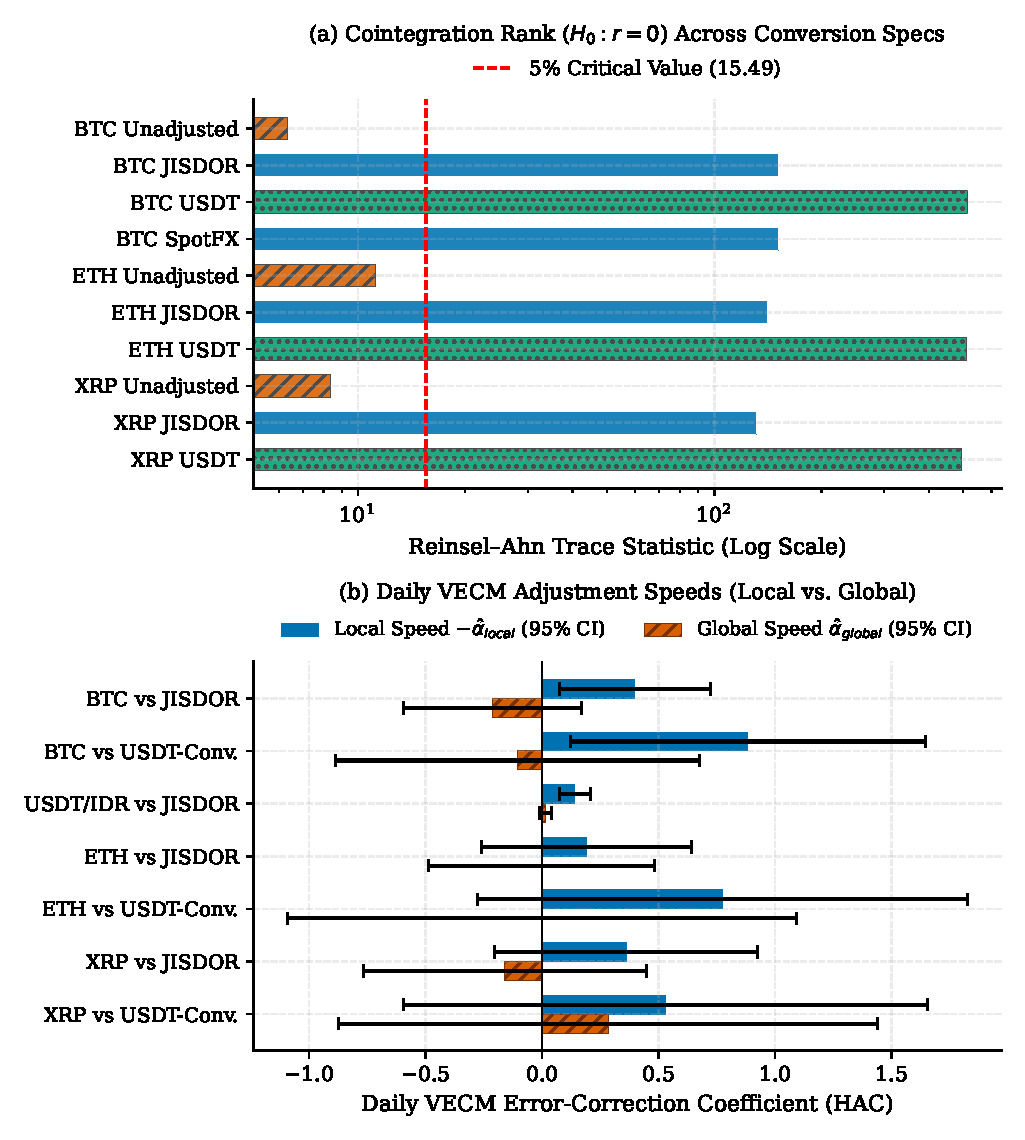
\includegraphics[width=\textwidth]{fig6_cointegration_and_ec.pdf}
  \caption{Unadjusted versus FX-converted Johansen trace statistics (Reinsel--Ahn, Panel~a) and daily VECM error-correction speeds with HAC 95\% confidence intervals (Panel~b).}
  \label{fig:ec}
\end{figure}

To analyze intraday price discovery without embedding domestic \texttt{USDT/IDR} into a synthetic global BTC price, Panel~B of Table~\ref{tab:vecm_ecm} estimates a three-variable five-minute VECM on the regular clock-time grid ($T_{eff} = 616,677$ equally spaced five-minute bars, five lagged differences, HAC $L = 12$) using $Y_t = [\ln P_{BTC,t}^{IDR},\, \ln P_{BTC,t}^{USDT},\, \ln U_t^{IDR/USDT}]'$. Both asymptotic Johansen rank tests ($\text{Trace}_{r=0} = 9,125.5$ vs.\ $5\%$ CV $29.80$; $\text{Trace}_{r\le 1} = 11.10$ vs.\ $15.49$) and the dependence-preserving block-wild bootstrap ($B = 499$, block length $b = 28$; $\text{Trace}_{r=0}$ bootstrap $p = 0.0020$ against $5\%$ bootstrap CV $56.19$) reject zero cointegration and support rank $r = 1$ with cointegrating vector $\hat{\beta} = [1.0000,\,-0.9994,\,-1.0045]'$.

Separating the three markets yields clear adjustment asymmetries, though cross-market price leadership remains bounded rather than uniquely identified. We fail to reject weak exogeneity for global Binance \texttt{BTC/USDT} ($\hat{\alpha}_{BTC/USDT} = +0.0011$, HAC SE $0.0014$, $p = 0.4179$), which accounts for $2.0\%$ of total error-correction adjustment. By contrast, Indodax \texttt{BTC/IDR} bears $80.0\%$ of error correction ($\hat{\alpha}_{BTC/IDR} = -0.0445$, HAC SE $0.0023$, $p < 0.0001$) and Indodax \texttt{USDT/IDR} bears the remaining $18.0\%$ ($\hat{\alpha}_{USDT/IDR} = +0.0100$, HAC SE $0.0007$, $p < 0.0001$). Inspecting the full companion matrix eigenvalues reveals a sharp spectral gap: the largest non-unit eigenvalue modulus is $|\lambda_{\max}| = 0.9728$ (implying a slowest-mode half-life of $25.08$ five-minute bars, compared with the scalar $1 + \beta'\alpha$ benchmark of $12.09$ bars), whereas the next-largest non-unit moduli are $\{0.5786, 0.5786\}$ (half-life $1.27$ bars), confirming that $|\lambda_{\max}| = 0.9728$ isolates the persistent error-correction mode rather than transient short-run lag dynamics. Across all six Cholesky orderings of $\Psi(1)$, Hasbrouck Information Share bounds for the permanent component of Indodax \texttt{BTC/IDR} span $[42.6\%, 99.0\%]$ for Binance \texttt{BTC/USDT}, $[1.0\%, 54.8\%]$ for Indodax \texttt{BTC/IDR}, and $[0.0\%, 3.0\%]$ for Indodax \texttt{USDT/IDR}; because the Binance and Indodax \texttt{BTC/IDR} bounds overlap, Hasbrouck shares indicate substantial global information transmission without uniquely isolating a single price leader.

Two sensitivity checks confirm the stability of this pattern. First, dropping the 11,533 zero-volume bars yields an irregularly spaced active-volume subsample ($T_{eff} = 605,150$) with similar adjustment shares ($80.3\%$ Indodax \texttt{BTC/IDR}, $1.3\%$ Binance \texttt{BTC/USDT}, $18.4\%$ Indodax \texttt{USDT/IDR}) but a faster active-bar companion half-life ($19.42$ active observations; scalar $9.25$), which should not be interpreted in regular five-minute clock units. Second, replacing Indodax \texttt{USDT/IDR} with Binance's native \texttt{USDT/IDR} over the 349-day overlap ($T_{eff} = 100,356$ regular bars) preserves non-rejection of weak exogeneity for global Binance \texttt{BTC/USDT} ($\hat{\alpha} = +0.0002$, HAC $p = 0.8580$; Hasbrouck IS $[25.0\%, 93.8\%]$), while Indodax \texttt{BTC/IDR} ($\hat{\alpha} = -0.0164$, HAC $p = 0.0001$, $48.0\%$ share) and Binance's thinner \texttt{USDT/IDR} book ($\hat{\alpha} = +0.0175$, HAC $p = 0.1833$, $51.3\%$ share) split domestic adjustment (companion half-life $22.17$ bars). Daily VECM residuals for \texttt{USDT/IDR}--JISDOR and five-minute BTC equations exhibit serial correlation and ARCH clustering ($\text{LB } p < 0.001$, $\text{ARCH } p < 0.001$), which motivates HAC standard errors for adjustment inference and our block-wild bootstrap for cointegration rank tests.

Threshold Band-TAR tests qualify the linear error-correction results across regimes. On daily $B_t^{crypto}$, the estimated threshold is $\hat{\tau} = 28.81\text{ bps}$, and the wild-bootstrap linearity test fails to reject linearity ($\sup W = 7.05$, $B = 499$, $p = 0.392$). By contrast, daily $B_t^{total}$ rejects linearity ($\hat{\tau} = 69.22\text{ bps}$, $\sup W = 72.92$, $p = 0.002$) with slower outer adjustment ($\hat{\rho}_{out} = -0.051$ vs.\ $\hat{\rho}_{in} = -0.390$, $13.25$-day outer half-life). At five-minute frequency, active-bar Band-TAR behavior varies by period: in an early 2022--2023 subsample ($n = 25,000$ active bars), linearity is rejected ($\hat{\tau} = 44.36\text{ bps}$, $\sup W = 202.38$, $B = 299$, $p = 0.0033$) with faster outer-band adjustment ($\hat{\rho}_{out} = -0.302$ vs.\ $\hat{\rho}_{in} = -0.080$, outer half-life $1.93$ bars), whereas in the recent 2026 subsample ($n = 25,000$ active bars), linearity is rejected ($\hat{\tau} = 17.81\text{ bps}$, $\sup W = 362.40$, $p = 0.0033$) with slower outer adjustment ($\hat{\rho}_{out} = -0.0115$ vs.\ $\hat{\rho}_{in} = -0.160$). Finally, in daily return dynamics ($n = 1,412$), contemporaneous regressions of $\Delta \ln P_t^{IDR}$ on $\Delta \ln P_t^{USDT}$, $\Delta \ln S_t^{FX}$, and $\Delta(\ln U_t - \ln S_t)$ hold nearly by accounting identity (Adjusted $R^2 > 0.99$); the informative non-mechanical test is the one-day lagged global crypto return, which carries a small positive catch-up coefficient of $+0.0212$ for BTC ($+0.0158$ ETH, $+0.0116$ XRP, all HAC $p < 0.0001$).

\subsection{Regulatory regimes, controlled event windows, and snapshot execution costs}
Table~\ref{tab:events} and Figure~\ref{fig:events} evaluate $\pm 30$-calendar-day event windows across ten regulatory, tax, and exchange-structure milestones from May 2022 through October 2026 \citep{pmk68_2022,binance_bidr_2024,indodax_events_2026,perba9_2024,pojk27_2024,pmk50_2025,cfx_seb001_2026,bi_padg072026}. Our primary inference uses $\pm 30$-day OLS regressions controlling for daily global BTC and JISDOR log returns with Newey--West HAC standard errors ($L=5$), with Holm multiple-testing adjustment applied across the 20-test BTC event $\times$ leg family. Because three event pairs overlap within $\pm 30$ calendar days and the October 31, 2026 maintenance event has only 12 post-event calendar days before our November 12, 2026 cutoff, Table~\ref{tab:events} also reports a simultaneous full-sample regression using non-overlapping $\pm 15$-day pre/post indicators.

\begin{table}[htbp]
\centering
\caption{30-Calendar-Day Pre/Post Institutional and Regulatory Event Windows (BTC Basis, bps)}
\label{tab:events}
\fontsize{6.3}{7.5}\selectfont\setlength{\tabcolsep}{2pt}
\begingroup
\begin{tabular}{@{}l>{\raggedright\arraybackslash}p{2.3cm}rrrrrr@{}}
\toprule
Date & Event & $\Delta\bar{B}^{cry}$ & $p_W$ ($p_{\text{Holm}}$) & $p_{\text{MW}}$ & $\Delta\bar{B}^{s\text{-}FX}$ & $p_W$ ($p_{\text{Holm}}$) & $p_{\text{MW}}$ \\
\midrule
2022-05-01 & PMK 68/2022 Tax & 13.23 & 0.293 (1.000) & 0.222 & 7.05 & 0.419 (1.000) & 0.066 \\
2024-05-17 & Binance BIDR Delist & 1.72 & 0.862 (1.000) & 0.502 & -0.54 & 0.951 (1.000) & 0.953 \\
2024-09-11 & Indodax Incident & -29.61 & 0.085 (1.000) & 0.162 & -14.25 & 0.045 (0.719) & 0.078 \\
2024-11-01 & CFX Fee Launch & -10.54 & 0.168 (1.000) & 0.232 & 14.45 & 0.018 (0.307) & 0.031 \\
2025-01-10 & OJK Transfer & 5.11 & 0.648 (1.000) & 0.574 & -13.79 & 0.102 (1.000) & 0.076 \\
2025-08-01 & PMK 50/2025 Tax & 21.23 & 0.0005 (0.011) & 0.002 & 14.08 & 0.014 (0.247) & 0.033 \\
2026-03-01 & CFX 1st 50\% Cut & -2.33 & 0.533 (1.000) & 0.804 & -3.73 & 0.423 (1.000) & 0.202 \\
2026-04-01 & JISDOR PADG 7/2026 & -1.71 & 0.615 (1.000) & 0.681 & -15.19 & 0.005 (0.090) & 0.008 \\
2026-10-01 & CFX 2nd 50\% Cut & 8.52 & 0.239 (1.000) & 0.432 & 7.73 & 0.186 (1.000) & 0.142 \\
2026-10-31 & Indodax Maintenance & -10.74 & 0.185 (1.000) & 0.421 & 11.68 & 0.071 (1.000) & 0.184 \\
\bottomrule
\end{tabular}\endgroup
\begin{minipage}{\textwidth}\footnotesize\vspace{3pt}
\emph{Notes:} $p_W$ and $p_{\text{MW}}$ are raw two-sided Welch $t$-test and Mann--Whitney $U$ $p$-values; $p_{\text{Holm}}$ is Holm-adjusted across all 20 event $\times$ leg tests. Under Mann--Whitney Holm adjustment, only PMK 50/2025 on $B^{cry}$ ($p_{\text{Holm}}=0.032$) is significant at 5\%. In OLS regressions over each $\pm 30$-day window controlling for daily BTC and JISDOR log returns (HAC $L=5$), PMK 50/2025 shifts $B^{cry}$ by $+17.22$ bps (raw $p=0.016$, Holm $p=0.275$) and CFX Fee Launch shifts $B^{s\text{-}FX}$ by $+17.37$ bps (raw $p=0.0013$, Holm $p=0.026$).
\end{minipage}
\end{table}


Two main findings emerge from comparing these specifications. First, under the primary $\pm 30$-day controlled HAC+Holm specification, the sole milestone surviving at the $5\%$ level is the \textbf{November 1, 2024 CFX/KKI bourse fee launch} on the stablecoin--FX leg $B_t^{stablecoin\text{-}FX}$, which shows a controlled post-event association of $+17.37\text{ bps}$ (HAC SE $5.40$, raw $p = 0.0013$, $p_{\text{Holm}} = 0.026$). Excluding the October 2--11, 2024 overlap with the Indodax security incident leaves this association virtually unchanged at $+17.23\text{ bps}$ (HAC SE $5.99$, $p = 0.0040$). Because $+17.37\text{ bps}$ is substantially larger than the $2.22$--$4.44\text{ bps}$ statutory CFX/KKI levy, it represents a post-event shift coincident with onshore stablecoin demand changes rather than a one-for-one fee pass-through; moreover, in the shorter non-overlapping $\pm 15$-day joint model, the association attenuates to $+10.89\text{ bps}$ ($p_{\text{Holm}} = 1.00$).

Second, the \textbf{August 1, 2025 PMK 50/2025 tax overhaul} on $B_t^{crypto}$ is specification-sensitive: in unadjusted Welch comparisons, $B_t^{crypto}$ shifts by $+21.23\text{ bps}$ ($p_{\text{Holm}} = 0.011$), but once controlling for daily BTC and JISDOR returns and serial correlation via HAC standard errors, it attenuates to $+17.22\text{ bps}$ (HAC SE $7.16$, raw $p = 0.016$) and does not survive Holm adjustment ($p_{\text{Holm}} = 0.275$). Conversely, the $\pm 15$-day joint model detects a sharp $+45.30\text{ bps}$ jump in $B_t^{crypto}$ around PMK 68/2022 ($p_{\text{Holm}} < 0.001$) that averages out over $\pm 30$ days ($+9.28\text{ bps}$, $p_{\text{Holm}} = 1.00$). Event-window magnitudes on $B_t^{crypto}$ and $B_t^{stablecoin\text{-}FX}$ are therefore sensitive to window length and return controls. In the single-day November 13, 2026 live limit-order book snapshot (Table~\ref{tab:fees} Panel~B), Route A incurs $66.46\text{ bps}$ all-in taker fee plus slippage at $\$1\text{k}$--$\$10\text{k}$ ($71.84\text{ bps}$ at $\$50\text{k}$) and pre-funded Route B incurs $76.46\text{ bps}$ at $\$10\text{k}$ ($81.85\text{ bps}$ at $\$50\text{k}$), whereas Route C via Indodax's thin \texttt{BTC/USDT} book incurs $153.36\text{ bps}$--$158.75\text{ bps}$ due to a $117.59\text{ bps}$ top-of-book spread. These figures measure point-in-time execution costs on November 13, 2026 rather than historical five-year depth.

\begin{figure}[htbp]
  \centering
  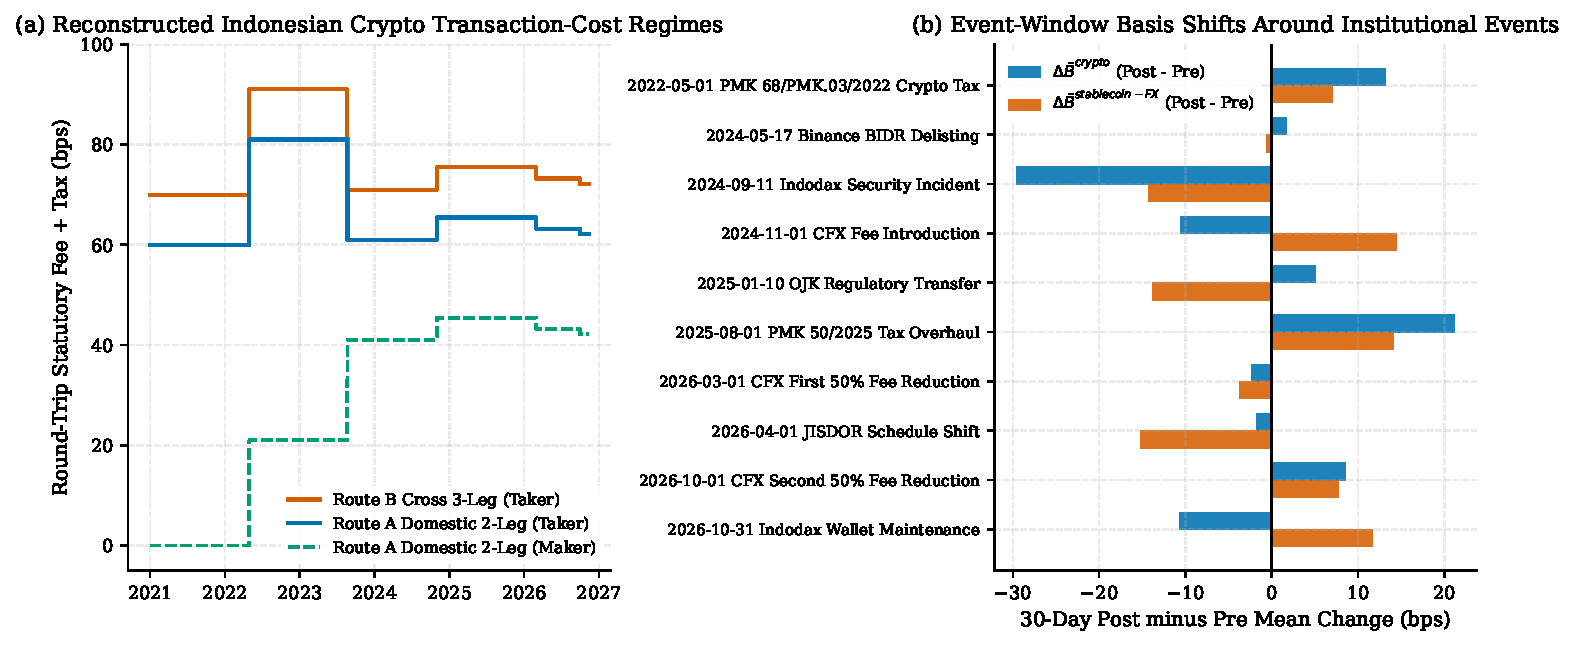
\includegraphics[width=\textwidth]{fig7_regulatory_and_costs.pdf}
  \caption{Reconstructed statutory execution cost bands across Routes A--B (Panel~a) and controlled HAC OLS $\pm 30$-day event-window basis shifts around ten institutional milestones (Panel~b; * denotes $p_{\text{Holm}} < 0.05$).}
  \label{fig:events}
\end{figure}
